\documentclass[calcdimensions,landscape,letterpaper]{powersem}
\usepackage{color}
\usepackage[pdftex]{thumbpdf} % For thumbnails
\usepackage[pdftex]{hyperref} % For links.
\usepackage[display,coloremph,whitebackground]{texpower} % colormath
\usepackage{fixseminar}
\usepackage{tpslifonts}
\usepackage[pdftex,final]{graphicx} % For including graphics.
\usepackage[utf8]{inputenc}
\usepackage{listings}
\usepackage{amsmath}
\usepackage{amssymb}
\usepackage{eurosym}
\usepackage{booktabs} % rules in tables
\usepackage{multirow} % multi-row cells
\usepackage{rotating} % text rotation

\title{The 5 SOLID Principles}
\author{Jan Wedekind}
\date{Thursday, Feb 22nd 2022}

\DeclareGraphicsExtensions{.jpg,.pdf,.png}
\pdfcompresslevel=9

\hypersetup{
   pdftitle          = {\thetitle},
   pdfsubject        = {After Catchup Presentation 22nd Feb 2022},
   pdfauthor         = {Jan Wedekind},
   pdfkeywords       = {},
   pdfcreator        = {okular},
   pdfproducer       = {LaTeX with hyperref and thumbpdf},
   bookmarksopen     = false,
   bookmarksnumbered = true,
   colorlinks        = true,
   pdfstartpage      = {1},
   pdfpagemode       = {FullScreen}
}

\lstset {
  language=Python,
  basicstyle=\tiny
}

% \textregistered for (R)
% \copyright for (C)
% \texttrademark for (TM) 

\DeclarePanel{top}{
  \begin{picture}(0,0)
    \put(82,-31){\parbox[c]{.5\textwidth}{\center\large\bf\thecurrentheading}}
  \end{picture}
}

\DeclarePanel{bottom}{
  \begin{picture}(0,0)
    \put(0,29){\parbox[c]{.98\pdfpagewidth}{\small\thedate\hfill\theslide}}
  \end{picture}
}

\slidesmag{4}
\backgroundstyle{none}
\slideframe{none}
\pagestyle{empty}

\mklength{\slideleftmargin}{-2cm}
\mklength{\sliderightmargin}{-2cm}
\mklength{\slidetopmargin}{4.5cm}
\mklength{\slidebottommargin}{2.37cm}

\renewcommand{\currentpagevalue}{\value{slide}}
\newcommand{\thecurrentheading}{}
\newcommand{\heading}[1]{\renewcommand{\thecurrentheading}{#1}}
\newcommand{\subheading}[1]{\concept{#1}}

\begin{document}

\begin{slide}
  \pdfbookmark[1]{\thetitle}{title}
  \heading{\thetitle}
  \begin{center}
    \maketitle
  \end{center}
\end{slide}

\begin{slide}
  \pdfbookmark[1]{Motivation}{motivation}
  \heading{Motivation}
  \begin{center}
    Maintain software quality over time as the project evolves!
  \end{center}
\end{slide}

\begin{slide}
  \pdfbookmark[1]{Software Rot}{software-rot}
  \heading{Software Rot}
  \begin{center}
    \textbf{Symptoms of rotting software design}\footnote{Robert C. Martin: Design Principles and Design Patterns}
    \begin{itemize}
      \item \textbf{Rigidity}: software difficult (a lot of work) to change
      \item \textbf{Fragility}: changes easily break the software
      \item \textbf{Immobility}: it is easier to rewrite than reuse parts of the software
      \item \textbf{Viscosity}: design preserving methods are harder to employ than hacks
    \end{itemize}
  \end{center}
\end{slide}

\begin{slide}
  \pdfbookmark[1]{Software Design}{software-design}
  \heading{Software Design}
  \begin{center}
    \begin{itemize}
      \item Keep software application \textbf{flexible}
      \item Keep software application \textbf{robust}
      \item Keep software application \textbf{reusable}
      \item Keep software application \textbf{developable}
    \end{itemize}
  \end{center}
\end{slide}

\begin{slide}
  \pdfbookmark[1]{Robert C. Martin}{robertmartin}
  \heading{Robert C. Martin aka "Uncle Bob"}
  \begin{center}
    \begin{minipage}[c]{.4\textwidth}
      \resizebox*{.93\textwidth}{!}{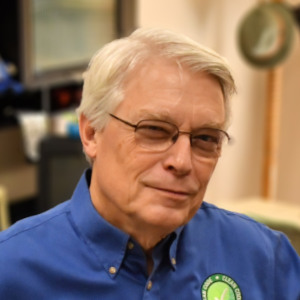
\includegraphics{robert-martin}}
    \end{minipage}
    \begin{minipage}[c]{.55\textwidth}
      \begin{itemize}
        \item Born 5.12.1952
        \item One of \href{https://agilemanifesto.org/}{Agile Manifesto}'s authors
        \item Author of \href{https://www.informit.com/store/clean-code-a-handbook-of-agile-software-craftsmanship-9780132350884}{Clean Code}, \href{https://www.informit.com/store/functional-design-principles-patterns-and-practices-9780138176396}{Functional Design}, and more books
        \item software consultant and trainer
        \item Author of \href{https://web.archive.org/web/20150906155800/http://www.objectmentor.com/resources/articles/Principles_and_Patterns.pdf}{Design Principles and Design Patterns} which later became SOLID
        \item Speaker at many conferences
        \item Advocate of Test-Driven Development
      \end{itemize}
    \end{minipage}
  \end{center}
\end{slide}

\begin{slide}
  \pdfbookmark[1]{The SOLID Principles}{solid-principles}
  \heading{The SOLID Principles}
  \begin{center}
    \begin{itemize}
      \item \textbf{S}ingle responsibility
      \item \textbf{O}pen-closed
      \item \textbf{L}iskov substitution
      \item \textbf{I}nterface segregation
      \item \textbf{D}ependency inversion
    \end{itemize}
  \end{center}
\end{slide}

\begin{slide}
  \pdfbookmark[1]{Listings Test}{listings-test}
  \heading{Listings Test}
  \begin{center}
    \begin{lstlisting}
def sqr(x):
    return x * x
    \end{lstlisting}
  \end{center}
\end{slide}

\begin{slide}
  \pdfbookmark[1]{The SOLID Principles}{solid-principles-2}
  \heading{The SOLID Principles}
  \begin{center}
    \begin{itemize}
      \item \textbf{S}ingle responsibility
      \item \textbf{O}pen-closed
      \item \textbf{L}iskov substitution
      \item \textbf{I}nterface segregation
      \item \textbf{D}ependency inversion
    \end{itemize}
  \end{center}
\end{slide}

\begin{slide}
  \pdfbookmark[1]{ArjanCodes video}{arjancodes-video}
  \heading{ArjanCodes: Uncle Bob's SOLID Principles Made Easy}
  \begin{center}
    \href{https://www.youtube.com/watch?v=pTB30aXS77U}{\resizebox*{.95\textwidth}{!}{
\includegraphics{arjancodes}}}
  \end{center}
\end{slide}

\end{document}
